\begin{tikzpicture}

% Waveform signal
\draw[
domain=0:9, 
samples=300,
smooth,
variable=\x,
blue,
ultra thick,
shift={(-4.5, 2.2)},
] plot ({\x},{sin((3.05*\x + 0.3) r) * 0.8});
\node at (0, 3.5) {\large Digital Waveform};
    
% Pressure wave
\node[
    label=south:{\large Acoustic Sound Wave}
] (pressure) at (0, 0) {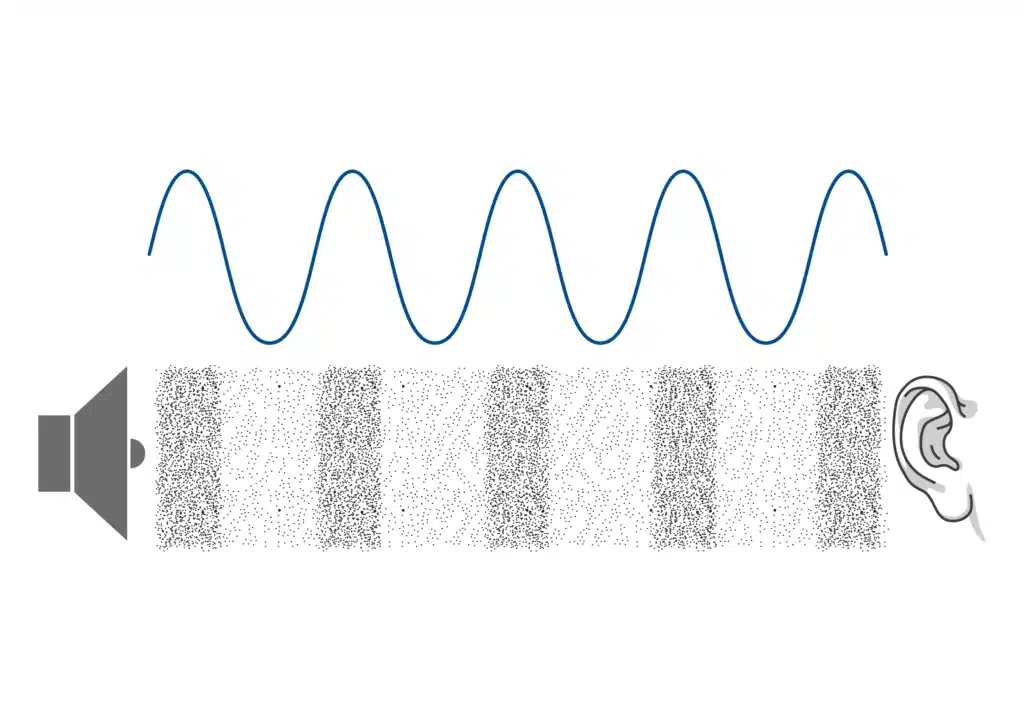
\includegraphics[trim={5.25cm 5.5cm 4.75cm 12.5cm},clip,scale=0.35]{figures/waveform}};

% Speaker
\node[left=-0.25cm of pressure] {
\includegraphics[scale=0.065]{figures/speaker.png}};

% Ear
\node[right=-0.25cm of pressure] {\scalebox{-1}[1]{
\includegraphics[scale=0.065]{figures/ear.png}}};

\end{tikzpicture}